\section[SPADE]{Smart Python Agent Development Environment (SPADE)}

\begin{frame}[fragile]{\insertsection}
    \begin{listing}
        \begin{mintedPython}
import spade

class DummyAgent(spade.agent.Agent):
    async def setup(self):
        print("Hello World! I'm agent {}".format(str(self.jid)))

async def main():
    dummy = DummyAgent("your_jid@your_xmpp_server", "your_password")
    await dummy.start()

if __name__ == "__main__":
    spade.run(main())
        \end{mintedPython}
        \caption{A simple SPADE agent}
    \end{listing}
\end{frame}

\begin{frame}{\insertsection}
    \customFigure[1]{
        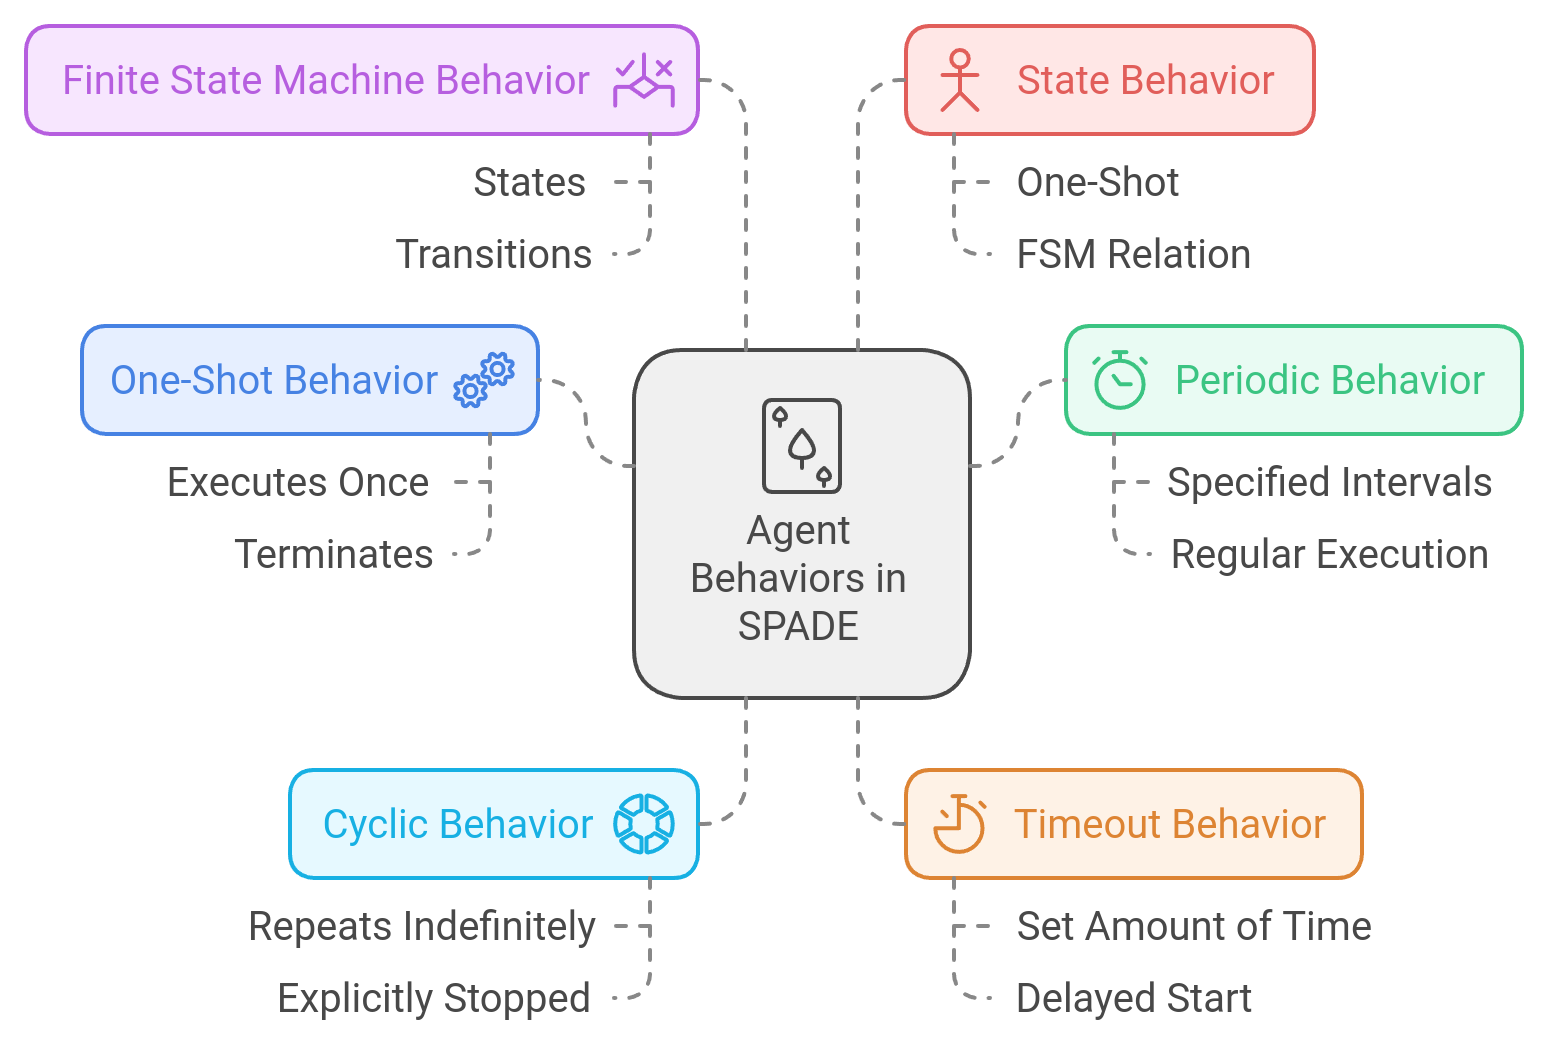
\includegraphics{Documents/241018 AI2Future/Figures/Agent behaviours in SPADE.png}
    }{Types of agent behaviour in SPADE}{agent agent behaviour}
\end{frame}


\begin{frame}[fragile]{\insertsection}
    \begin{listing}
        \begin{mintedPython}
class DummyAgent(Agent):
    class MyBehav(CyclicBehaviour):
        async def on_start(self):
            print("Starting behaviour . . .")

        async def run(self):
            print("Running the behaviour . . .")

    async def setup(self):
        print("Agent starting . . .")
        b = self.MyBehav()
        self.add_behaviour(b)

async def main():
    dummy = DummyAgent("your_jid@your_xmpp_server", "your_password")
    await dummy.start()

    await wait_until_finished(dummy)
        \end{mintedPython}
        \caption{A simple SPADE agent with a simple cyclic behaviour}
    \end{listing}
\end{frame}

\begin{frame}{\insertsection}
    \customFigure[0.8]{
        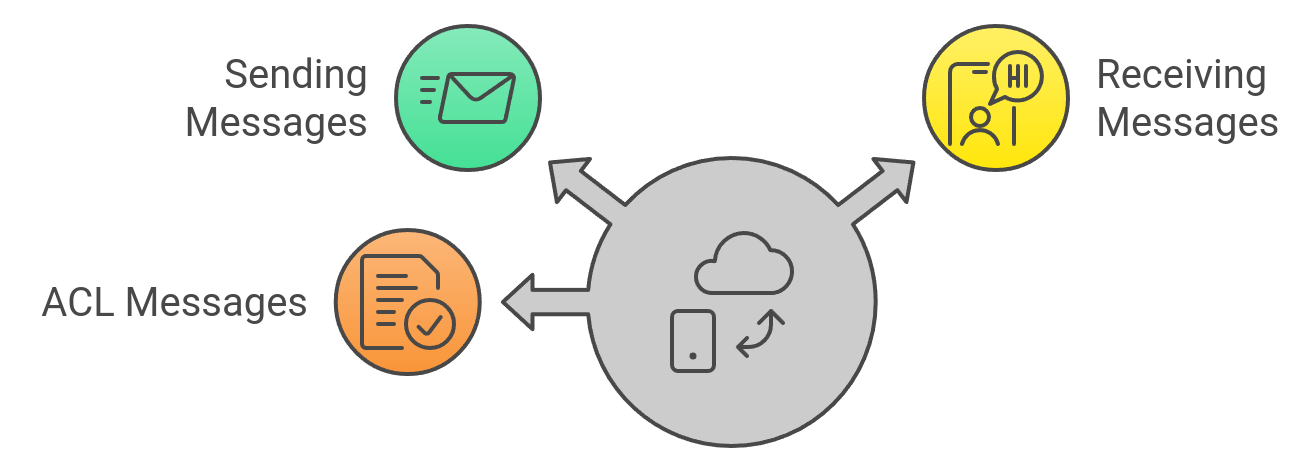
\includegraphics{Documents/241018 AI2Future/Figures/Agent communication.png}
    }{Features of agent communication in SPADE}{agent communication}
\end{frame}

\begin{frame}[fragile]{\insertsection}
    \begin{listing}
        \begin{mintedPython}
    class ReceiverAgent(Agent):
        class ReceiveBehav(OneShotBehavior):
            async def run(self):
                msg = await self.receive(timeout=10)
                if msg:
                    print(f"Message received: {msg.body}")
                else:
                    print("No message received.")
    
    async def setup(self):
        print("Receiver Agent is starting...")
        self.add_behaviour(self.ReceiveBehav())
        \end{mintedPython}
        \caption{Implementing an agent that can receive messages.}
    \end{listing}
\end{frame}


\begin{frame}[fragile]{\insertsection}
    \begin{listing}
        \begin{mintedPython}
class SenderAgent(Agent):
    class SendBehav(OneShotBehavior):
        async def run(self):
            msg = Message(to="receiver@your_xmpp_server")
            msg.set_metadata("performative", "inform")
            msg.body = "Hello, Agent B!"
            await self.send(msg)
            print("Message sent!")

    async def setup(self):
        print("Sender Agent is starting...")
        self.add_behaviour(self.SendBehav())
        \end{mintedPython}
        \caption{Implementing an agent that can send messages.}
    \end{listing}
\end{frame}
